%% LyX 2.3.0 created this file.  For more info, see http://www.lyx.org/.
%% Do not edit unless you really know what you are doing.
\documentclass[ruled]{article}
\usepackage{courier}
\usepackage[T1]{fontenc}
\usepackage[latin9]{inputenc}
\usepackage[letterpaper]{geometry}
\geometry{verbose}
\usepackage{color}
\usepackage{algorithm2e}
\usepackage{amsmath}
\usepackage{amssymb}
\usepackage{graphicx}
\usepackage[unicode=true,
 bookmarks=false,
 breaklinks=false,pdfborder={0 0 1},backref=section,colorlinks=true]
 {hyperref}

\makeatletter

%%%%%%%%%%%%%%%%%%%%%%%%%%%%%% LyX specific LaTeX commands.
\providecommand{\LyX}{\texorpdfstring%
  {L\kern-.1667em\lower.25em\hbox{Y}\kern-.125emX\@}
  {LyX}}
%% Special footnote code from the package 'stblftnt.sty'
%% Author: Robin Fairbairns -- Last revised Dec 13 1996
\let\SF@@footnote\footnote
\def\footnote{\ifx\protect\@typeset@protect
    \expandafter\SF@@footnote
  \else
    \expandafter\SF@gobble@opt
  \fi
}
\expandafter\def\csname SF@gobble@opt \endcsname{\@ifnextchar[%]
  \SF@gobble@twobracket
  \@gobble
}
\edef\SF@gobble@opt{\noexpand\protect
  \expandafter\noexpand\csname SF@gobble@opt \endcsname}
\def\SF@gobble@twobracket[#1]#2{}
%% Because html converters don't know tabularnewline
\providecommand{\tabularnewline}{\\}

\@ifundefined{date}{}{\date{}}
%%%%%%%%%%%%%%%%%%%%%%%%%%%%%% User specified LaTeX commands.
\definecolor{mygreen}{rgb}{0,0.6,0}
\definecolor{mygray}{rgb}{0.5,0.5,0.5}
\definecolor{mymauve}{rgb}{0.58,0,0.82}

\makeatother

\begin{document}
\global\long\def\reals{\mathbf{R}}
 \global\long\def\integers{\mathbf{Z}}
\global\long\def\naturals{\mathbf{N}}
 \global\long\def\rationals{\mathbf{Q}}
\global\long\def\ca{\mathcal{A}}
\global\long\def\cb{\mathcal{B}}
 \global\long\def\cc{\mathcal{C}}
 \global\long\def\cd{\mathcal{D}}
\global\long\def\ce{\mathcal{E}}
\global\long\def\cf{\mathcal{F}}
\global\long\def\cg{\mathcal{G}}
\global\long\def\ch{\mathcal{H}}
\global\long\def\ci{\mathcal{I}}
\global\long\def\cj{\mathcal{J}}
\global\long\def\ck{\mathcal{K}}
\global\long\def\cl{\mathcal{L}}
\global\long\def\cm{\mathcal{M}}
\global\long\def\cn{\mathcal{N}}
\global\long\def\co{\mathcal{O}}
\global\long\def\cp{\mathcal{P}}
\global\long\def\cq{\mathcal{Q}}
\global\long\def\calr{\mathcal{R}}
\global\long\def\cs{\mathcal{S}}
\global\long\def\ct{\mathcal{T}}
\global\long\def\cu{\mathcal{U}}
\global\long\def\cv{\mathcal{V}}
\global\long\def\cw{\mathcal{W}}
\global\long\def\cx{\mathcal{X}}
\global\long\def\cy{\mathcal{Y}}
\global\long\def\cz{\mathcal{Z}}
\global\long\def\ind#1{1(#1)}
\global\long\def\pr{\mathbb{P}}

\global\long\def\ex{\mathbb{E}}
\global\long\def\var{\textrm{Var}}
\global\long\def\cov{\textrm{Cov}}
\global\long\def\sgn{\textrm{sgn}}
\global\long\def\sign{\textrm{sign}}
\global\long\def\kl{\textrm{KL}}
\global\long\def\law{\mathcal{L}}
\global\long\def\eps{\varepsilon}
\global\long\def\convd{\stackrel{d}{\to}}
\global\long\def\eqd{\stackrel{d}{=}}
\global\long\def\del{\nabla}
\global\long\def\loss{\ell}
\global\long\def\tr{\operatorname{tr}}
\global\long\def\trace{\operatorname{trace}}
\global\long\def\diag{\text{diag}}
\global\long\def\rank{\text{rank}}
\global\long\def\linspan{\text{span}}
\global\long\def\proj{\text{Proj}}
\global\long\def\argmax{\operatornamewithlimits{arg\, max}}
\global\long\def\argmin{\operatornamewithlimits{arg\, min}}
\global\long\def\bfx{\mathbf{x}}
\global\long\def\bfy{\mathbf{y}}
\global\long\def\bfl{\mathbf{\lambda}}
\global\long\def\bfm{\mathbf{\mu}}
\global\long\def\calL{\mathcal{L}}
\global\long\def\vw{\boldsymbol{w}}
\global\long\def\vx{\boldsymbol{x}}
\global\long\def\vxi{\boldsymbol{\xi}}
\global\long\def\valpha{\boldsymbol{\alpha}}
\global\long\def\vbeta{\boldsymbol{\beta}}
\global\long\def\vsigma{\boldsymbol{\sigma}}
\global\long\def\vmu{\boldsymbol{\mu}}
\global\long\def\vtheta{\boldsymbol{\theta}}
\global\long\def\vd{\boldsymbol{d}}
\global\long\def\vs{\boldsymbol{s}}
\global\long\def\vt{\boldsymbol{t}}
\global\long\def\vh{\boldsymbol{h}}
\global\long\def\ve{\boldsymbol{e}}
\global\long\def\vf{\boldsymbol{f}}
\global\long\def\vg{\boldsymbol{g}}
\global\long\def\vz{\boldsymbol{z}}
\global\long\def\vk{\boldsymbol{k}}
\global\long\def\va{\boldsymbol{a}}
\global\long\def\vb{\boldsymbol{b}}
\global\long\def\vv{\boldsymbol{v}}
\global\long\def\vy{\boldsymbol{y}}
\global\long\def\nll{\text{NLL}}


\title{Homework 5: Conditional Probability Models}

\maketitle
\textbf{Instructions}: Your answers to the questions below, including
plots and mathematical work, should be submitted as a single PDF file.
It's preferred that you write your answers using software that typesets
mathematics (e.g. \LaTeX , \LyX , or MathJax via iPython), though
if you need to you may scan handwritten work. You may find the \href{https://github.com/gpoore/minted}{minted}
package convenient for including source code in your \LaTeX{} document.
If you are using \LyX , then the \href{https://en.wikibooks.org/wiki/LaTeX/Source_Code_Listings}{listings}
package tends to work better.

\section{Introduction }

In this homework we'll be investigating conditional probability models,
with a focus on various interpretations of logistic regression, with
and without regularization. Along the way we'll discuss the calibration
of probability predictions, both in the limit of infinite training
data and in a more bare-hands way. On the Bayesian side, we'll recreate
from scratch the Bayesian linear gaussian regression example we discussed
in lecture. We'll also have several optional problems that work through
many basic concepts in Bayesian statistics via one of the simplest
problems there is: estimating the probability of heads in a coin flip.
Later we'll extend this to the probability of estimating click-through
rates in mobile advertising. Along the way we'll encounter empirical
Bayes and hierarchical models. 

\section{From Scores to Conditional Probabilities\protect\footnote{This problem is based on Section 7.5.3 of Schapire and Freund's book
\emph{Boosting: Foundations and Algorithms}.}}

Let's consider the classification setting, in which $\left(x_{1},y_{1}\right),\ldots,\left(x_{n},y_{n}\right)\in\cx\times\left\{ -1,1\right\} $
are sampled i.i.d. from some unknown distribution. For a prediction
function $f:\cx\to\reals$, we define the \textbf{margin }on an example
$\left(x,y\right)$ to be $m=yf(x)$. Since our class predictions
are given by $\sign(f(x))$, we see that a prediction is correct iff
$m(x)>0$. It's tempting to interpret the magnitude of the score $\left|f(x)\right|$
as a measure of confidence. However, it's hard to interpret the magnitudes
beyond saying one prediction score is more or less confident than
another, and without any scale to this ``confidence score'', it's
hard to know what to do with it. In this problem, we investigate how
we can translate the score into a probability, which is much easier
to interpret. In other words, we are looking for a way to convert
score function $f(x)\in\reals$ into a conditional probability distribution
$x\mapsto p(y=1\mid x)$. 

In this problem we will consider \textbf{margin-based losses}, which
are loss functions of the form $\left(y,f(x)\right)\mapsto\ell\left(yf(x)\right)$,
where $m=yf(x)$ is called the \textbf{margin}. We are interested
in how we can go from an empirical risk minimizer for a margin-based
loss, $\hat{f}=\argmin_{f\in\cf}\sum_{i=1}^{n}\ell\left(y_{i}f(x_{i})\right)$,
to a conditional probability estimator $\hat{\pi}(x)\approx p(y=1\mid x)$.
Our approach will be to try to find a way to use the Bayes\footnote{Don't be confused -- it's Bayes as in ``Bayes optimal'', as we
discussed at the beginning of the course, not Bayesian as we've discussed
more recently.} prediction function\footnote{In this context, the Bayes prediction function is often referred to
as the ``population minimizer.'' In our case, ``population'' refers
to the fact that we are minimizing with respect to the true distribution,
rather than a sample. The term ``population'' arises from the context
where we are using a sample to approximate some statistic of an entire
population (e.g. a population of people or trees).} $f^{*}=\argmin_{f}\ex_{x,y}\left[\ell(yf(x)\right]$ to get the true
conditional probability $\pi(x)=p(y=1\mid x$), and then apply the
same mapping to the empirical risk minimizer. While there is plenty
that can go wrong with this ``plug-in'' approach (primarily, the
empirical risk minimizer from a {[}limited{]} hypothesis space $\cf$
may be a poor estimate for the Bayes prediction function), it is at
least well-motivated, and it can work well in practice. And \textbf{please
note} that we can do better than just hoping for success: if you have
enough validation data, you can directly assess how well ``calibrated''
the predicted probabilities are. This blog post has some discussion
of calibration plots: \href{https://jmetzen.github.io/2015-04-14/calibration.html}{https://jmetzen.github.io/2015-04-14/calibration.html}. 

It turns out it is straightforward to find the Bayes prediction function
$f^{*}$ for margin losses, at least in terms of the data-generating
distribution: For any given $x\in\cx$, we'll find the best possible
prediction $\hat{y}$. This will be the $\hat{y}$ that minimizes
\[
\ex_{y}\left[\ell\left(y\hat{y}\right)\mid x\right].
\]
If we can calculate this $\hat{y}$ for all $x\in\cx$, then we will
have determined $f^{*}(x)$. We will simply take
\[
f^{*}(x)=\argmin_{\hat{y}}\ex_{y}\left[\ell\left(y\hat{y}\right)\mid x\right].
\]

Below we'll calculate $f^{*}$ for several loss functions. It will
be convenient to let $\pi(x)=p\left(y=1\mid x\right)$ in the work
below. 
\begin{enumerate}
\item Write $\ex_{y}\left[\ell\left(yf(x)\right)\mid x\right]$ in terms
of $\pi(x)$, $\ell(-f(x))$, and $\ell\left(f(x)\right)$. {[}Hint:
Use the fact that $y\in\left\{ -1,1\right\} $.{]}
\item Show that the Bayes prediction function $f^{*}(x)$ for the exponential
loss function $\ell\left(y,f(x)\right)=e^{-yf(x)}$ is given by 
\[
f^{*}(x)=\frac{1}{2}\ln\left(\frac{\pi(x)}{1-\pi(x)}\right),
\]
where we've assumed $\pi(x)\in\left(0,1\right)$. Also, show that
given the Bayes prediction function $f^{*}$, we can recover the conditional
probabilities by
\[
\pi(x)=\frac{1}{1+e^{-2f^{*}(x)}}.
\]
{[}Hint: Differentiate the expression in the previous problem with
respect to $f(x)$. To make things a little less confusing, and also
to write less, you may find it useful to change variables a bit: Fix
an $x\in\cx$. Then write $p=\pi(x)$ and $\hat{y}=f(x)$. After substituting
these into the expression you had for the previous problem, you'll
want to find $\hat{y}$ that minimizes the expression. Use differential
calculus. Once you've done it for a single $x$, it's easy to write
the solution as a function of $x$.{]} 
\item Show that the Bayes prediction function $f^{*}(x)$ for the logistic
loss function $\ell\left(y,f(x)\right)=\ln\left(1+e^{-yf(x)}\right)$
is given by
\[
f^{*}(x)=\ln\left(\frac{\pi(x)}{1-\pi(x)}\right)
\]
and the conditional probabilities are given by
\[
\pi(x)=\frac{1}{1+e^{-f^{*}(x)}}.
\]
 Again, we may assume that $\pi(x)\in(0,1)$.
\item {[}Optional{]} Show that the Bayes prediction function $f^{*}(x)$
for the hinge loss function $\ell\left(y,f(x)\right)=\max\left(0,1-yf(x)\right)$
is given by
\[
f^{*}(x)=\sign\left(\pi(x)-\frac{1}{2}\right).
\]
Note that it is impossible to recover $\pi(x)$ from $f^{*}(x)$ in
this scenario. However, in practice we work with an empirical risk
minimizer, from which we may still be able to recover a reasonable
estimate for $\pi(x)$. An early approach to this problem is known
as ``Platt scaling'': \href{https://en.wikipedia.org/wiki/Platt_scaling}{https://en.wikipedia.org/wiki/Platt\_scaling}.
\end{enumerate}

\section{Logistic Regression}

\subsection{\label{subsec:erm-bernoulli-setup}Equivalence of ERM and probabilistic
approaches}

In lecture we discussed two different ways to end up with logistic
regression. 

\textbf{ERM approach:} Consider the classification setting with input
space $\cx=\reals^{d}$, outcome space $\cy_{\pm}=\left\{ -1,1\right\} $,
and action space $\ca_{\text{\ensuremath{\reals}}}=\reals$, with
the hypothesis space of linear score functions $\cf_{\text{score}}=\left\{ x\mapsto x^{T}w\mid w\in\reals^{d}\right\} $.
Consider the margin-based loss function $\ell_{\text{logistic}}(m)=\log\left(1+e^{-m}\right)$
and the training data $\cd=\left((x_{1},y_{1}),\ldots,(x_{n},y_{n})\right)$.
Then the empirical risk objective function for hypothesis space $\cf_{\text{score}}$
and the logistic loss over $\cd$ is given by

\begin{eqnarray*}
\hat{R}_{n}(w) & = & \frac{1}{n}\sum_{i=1}^{n}\ell_{\text{logistic}}(y_{i}w^{T}x_{i})\\
 & = & \frac{1}{n}\sum_{i=1}^{n}\log\left(1+\exp\left(-y_{i}w^{T}x_{i}\right)\right).
\end{eqnarray*}
 

\textbf{Bernoulli regression with logistic transfer function:} Consider
the conditional probability modeling setting with input space $\cx=\reals^{d}$,
outcome space $\cy_{0/1}=\left\{ 0,1\right\} $, and action space
$\ca_{[0,1]}=[0,1]$, where an action corresponds to the predicted
probability that an outcome is $1$. Define the \textbf{standard logistic
function} as $\phi(\eta)=1/\left(1+e^{-\eta}\right)$ and the hypothesis
space $\cf_{\text{prob}}=\left\{ x\mapsto\phi(w^{T}x)\mid w\in\reals^{d}\right\} $.
Suppose for every $y_{i}$ in the dataset $\cd$ above, we define
$y_{i}'=\begin{cases}
1 & y_{i}=1\\
0 & y_{i}=-1
\end{cases}$, and let $\cd'$ be the resulting collection of $\left(x_{i},y_{i}'\right)$
pairs. Then the negative log-likelihood (NLL) objective function for
$\cf_{\text{prob}}$ and $\cd'$ is give by 
\begin{eqnarray*}
\nll(w) & = & -\sum_{i=1}^{n}y_{i}'\log\phi(w^{T}x_{i})+\left(1-y_{i}'\right)\log\left(1-\phi(w^{T}x_{i})\right)\\
 & = & \sum_{i=1}^{n}\left[-y_{i}'\log\phi(w^{T}x_{i})\right]+\left(y_{i}'-1\right)\log\left(1-\phi(w^{T}x_{i})\right)
\end{eqnarray*}
If $\hat{w}_{\text{prob}}$ minimizes $\nll(w)$, then $x\mapsto\phi(x^{T}\hat{w}_{\text{prob}})$
is a maximum likelihood prediction function over the hypothesis space
$\cf_{\text{prob}}$ for the dataset $\cd'$. 

\textbf{Show that} $n\hat{R}_{n}(w)=\nll(w)$ for all $w\in\reals^{d}$.
And thus the two approaches are equivalent, in that they produce the
same prediction functions.

\subsection{Numerical Overflow and the log-sum-exp trick}

Suppose we want to calculate $\log\left(\exp(\eta)\right)$ for $\eta=1000.42$.
If we compute this literally in Python, we will get an overflow (try
it!), since numpy gets infinity for $e^{1000.42}$, and log of infinity
is still infinity. On the other hand, we can help out with some math:
obviously $\log\left(\exp(\eta)\right)=\eta$, and there's no issue. 

It turns out, $\log(\exp(\eta))$ and the problem with its calculation
is a special case of the \href{https://en.wikipedia.org/wiki/LogSumExp}{LogSumExp}
function that shows up frequently in machine learning. We define
\[
\text{LogSumExp}(x_{1},\ldots,x_{n})=\log\left(e^{x_{1}}+\cdots+e^{x_{n}}\right).
\]
Note that this will overflow if any of the $x_{i}$'s are large (more
than 709). To compute this on a computer, we can use the ``\textbf{log-sum-exp
trick}''. We let $x^{*}=\max\left(x_{1},\ldots,x_{n}\right)$ and
compute LogSumExp as
\[
\text{LogSumExp}(x_{1},\ldots,x_{n})=x^{*}+\log\left[e^{x_{1}-x^{*}}+\cdots+e^{x_{n}-x^{*}}\right].
\]

\begin{enumerate}
\item Show that the new expression for LogSumExp is valid.
\item Show that $\exp\left(x_{i}-x^{*}\right)\in(0,1]$ for any $i$, and
thus the exp calculations will not overflow. 
\item Above we've only spoken about the exp overflowing. However, the log
part can also have problems by becoming negative infinity for arguments
very close to $0$. Explain why the $\log$ term in our expression
$\log\left[e^{x_{1}-x^{*}}+\cdots+e^{x_{n}-x^{*}}\right]$ will never
be ``-inf''. 
\item In the objective functions for logistic regression, there are expressions
of the form $\log\left(1+e^{-s}\right)$ for some $s$. Note that
a naive implementation gives $0$ for $s>36$ and inf for $s<-709$.
Show how to use the numpy function\textit{ \href{https://docs.scipy.org/doc/numpy/reference/generated/numpy.logaddexp.html}{logaddexp}
}\textit{\emph{to correctly compute $\log\left(1+e^{-s}\right)$.
}} 
\end{enumerate}

\subsection{\label{subsec:Regularized-Logistic-Regression}Regularized Logistic
Regression}

For a dataset $\cd=\left((x_{1},y_{1}),\ldots,(x_{n},y_{n})\right)$
drawn from $\reals^{d}\times\left\{ -1,1\right\} $, the regularized
logistic regression objective function can be defined as
\begin{eqnarray*}
J_{\text{logistic}}(w) & = & \hat{R}_{n}(w)+\lambda\|w\|^{2}\\
 & = & \frac{1}{n}\sum_{i=1}^{n}\log\left(1+\exp\left(-y_{i}w^{T}x_{i}\right)\right)+\lambda\|w\|^{2}.
\end{eqnarray*}
 
\begin{enumerate}
\item Prove that the objective function $J_{\text{logistic}}(w)$ is convex.
You may use any facts mentioned in the \href{https://davidrosenberg.github.io/mlcourse/Notes/convex-optimization.pdf}{convex optimization notes}.
\item Complete the \texttt{f\_objective} function in the skeleton code,
which computes the objective function for $J_{\text{logistic}}(w)$.
Make sure to use the log-sum-exp trick to get accurate calculations
and to prevent overflow.
\item Complete the \texttt{fit\_logistic\_regression\_function} in the skeleton
code using the \texttt{minimize} function from \texttt{scipy.optimize}.
\texttt{ridge\_regression.py} from Homework 2 gives an example of
how to use the \texttt{minimize} function. Use this function to train
a model on the provided data. Make sure to take the appropriate preprocessing
steps, such as standardizing the data and adding a column for the
bias term. 
\item Find the $\ell_{2}$ regularization parameter that minimizes the log-likelihood
on the validation set. Plot the log-likelihood for different values
of the regularization parameter. 
\item Based on the Bernoulli regression development of logistic regression,
it seems reasonable to interpret the prediction $f(x)=\phi(w^{T}x)=1/\left(1+e^{-w^{T}x}\right)$
as the probability that $y=1$, for a randomly drawn pair $\left(x,y\right)$.
Since we only have a finite sample (and we are regularizing, which
will bias things a bit) there is a question of how well ``\href{https://en.wikipedia.org/wiki/Calibration_(statistics)}{calibrated}''
our predicted probabilities are. Roughly speaking, we say $f(x)$
is well calibrated if we look at all examples $\left(x,y\right)$
for which $f(x)\approx0.7$ and we find that close to $70\%$ of those
examples have $y=1$, as predicted... and then we repeat that for
all predicted probabilities in $\left(0,1\right)$. To see how well-calibrated
our predicted probabilities are, break the predictions on the validation
set into groups based on the predicted probability (you can play with
the size of the groups to get a result you think is informative).
For each group, examine the percentage of positive labels. You can
make a table or graph. Summarize the results. You may get some ideas
and references from \href{http://scikit-learn.org/stable/modules/calibration.html}{scikit-learn's discussion}. 
\item {[}Optional{]} If you can, create a dataset for which the log-sum-exp
trick is actually necessary for your implementation of regularized
logistic regression. If you don't think such a dataset exists, explain
why. If you like, you may consider the case of SGD optimization. {[}This
problem is intentionally open-ended. You're meant to think, explore,
and experiment. Points assigned for interesting insights.{]}
\end{enumerate}

\section{Bayesian Logistic Regression with Gaussian Priors}

Let's return to the setup described in Section \ref{subsec:erm-bernoulli-setup}
and, in particular, to the Bernoulli regression setting with logistic
transfer function. We had the following hypothesis space of conditional
probability functions:
\[
\cf_{\text{prob}}=\left\{ x\mapsto\phi(w^{T}x)\mid w\in\reals^{d}\right\} .
\]
Now let's consider the Bayesian setting, where we induce a prior on
$\cf_{\text{prob}}$ by taking a prior $p(w)$ on the parameter $w\in\reals^{d}$. 
\begin{enumerate}
\item For the dataset $\cd'$ described in Section \ref{subsec:erm-bernoulli-setup},
give an expression for the posterior density $p(w\mid\cd')$ in terms
of the negative log-likelihood function 
\begin{eqnarray*}
\nll_{\cd'}(w) & = & -\sum_{i=1}^{n}y_{i}'\log\phi(w^{T}x_{i})+\left(1-y_{i}'\right)\log\left(1-\phi(w^{T}x_{i})\right)
\end{eqnarray*}
and a prior density $p(w)$ (up to a proportionality constant is fine).
\item Suppose we take a prior on $w$ of the form $w\sim\cn(0,\Sigma)$.
Find a covariance matrix $\Sigma$ such that MAP estimate for $w$
after observing data $\cd'$ is the same as the minimizer of the regularized
logistic regression function defined in Section \ref{subsec:Regularized-Logistic-Regression}
(and prove it). {[}Hint: Consider minimizing the negative log posterior
of $w$. Also, remember you can drop any terms from the objective
function that don't depend on $w$. Also, you may freely use results
of previous problems.{]}
\item In the Bayesian approach, the prior should reflect your beliefs about
the parameters before seeing the data and, in particular, should be
independent on the eventual size of your dataset. Following this,
you choose a prior distribution $w\sim\cn(0,I)$. For a dataset $\cd$
of size $n$, how should you choose $\lambda$ in our regularized
logistic regression objective function so that the minimizer is equal
to the mode of the posterior distribution of $w$ (i.e. is equal to
the MAP estimator). 
\end{enumerate}

\section{Bayesian Linear Regression - Implementation}

In this problem, we will implement Bayesian Gaussian linear regression,
essentially reproducing the example \href{https://davidrosenberg.github.io/mlcourse/Archive/2016/Lectures/13a.bayesian-regression.pdf\#page=12}{from lecture},
which in turn is based on the example in Figure 3.7 of Bishop's \emph{Pattern
Recognition and Machine Learning} (page 155). We've provided plotting
functionality in \textquotedbl support\_code.py\textquotedbl . Your
task is to complete \textquotedbl problem.py\textquotedbl . The
implementation uses np.matrix objects, and you are welcome to use\footnote{However, in practice we are usually interested in computing the product
of a matrix inverse and a vector, i.e. $X^{-1}b$. In this case, it's
usually faster and more accurate to use a library's algorithms for
solving a system of linear equations. Note that $y=X^{-1}b$ is just
the solution to the linear system $Xy=b$. See for example \href{https://www.johndcook.com/blog/2010/01/19/dont-invert-that-matrix/}{John Cook's blog post}
for discussion. } the np.matrix.getI method. 
\begin{enumerate}
\item Implement likelihood\_func.
\item Implement get\_posterior\_params.
\item Implement get\_predictive\_params.
\item Run ``python problem.py'' from inside the Bayesian Regression directory
to do the regression and generate the plots. This runs through the
regression with three different settings for the prior covariance.
You may want to change the default behavior in support\_code.make\_plots
from plt.show, to saving the plots for inclusion in your homework
submission.
\item Comment on your results. In particular, discuss how each of the following
change with sample size and with the strength of the prior:  (i) the
likelihood function, (ii) the posterior distribution, and (iii) the
posterior predictive distribution.
\item Our work above was very much ``full Bayes'', in that rather than
coming up with a single prediction function, we have a whole distribution
over posterior prediction functions. However, sometimes we want a
single prediction function, and a common approach is to use the MAP
estimate -- that is, choose the prediction function that has the
highest posterior likelihood. As we discussed in class, for this setting,
we can get the MAP estimate using ridge regression. Use ridge regression
to get the MAP prediction function corresponding to the first prior
covariance ($\Sigma=\frac{1}{2}I$, per the support code). What value
did you use for the regularization coefficient? Why? 
\end{enumerate}

\section{{[}Optional{]} Coin Flipping: Maximum Likelihood}
\begin{enumerate}
\item {[}Optional{]} Suppose we flip a coin and get the following sequence
of heads and tails:
\[
\cd=(H,H,T)
\]
Give an expression for the probability of observing $\cd$ given that
the probability of heads is $\theta$. That is, give an expression
for $p\left(\cd\mid\theta\right)$. This is called the \textbf{likelihood
of $\theta$ for the data $\cd$}.\\
\item {[}Optional{]} How many different sequences of 3 coin tosses have
$2$ heads and 1 tail? If we toss the coin $3$ times, what is the
probability of 2 heads and $1$ tail? (Answer should be in terms of
$\theta$.)\\
\item {[}Optional{]} More generally, give an expression for the likelihood
$p(\cd\mid\theta)$ for a particular sequence of flips $\cd$ that
has $n_{h}$ heads and $n_{t}$ tails. Make sure you have expressions
that make sense even for $\theta=0$ and $n_{h}=0$, and other boundary
cases. You may use the convention that $0^{0}=1$, or you can break
your expression into cases if needed.\\
\item {[}Optional{]} Show that the maximum likelihood estimate of $\theta$
given we observed a sequence with $n_{h}$ heads and $n_{t}$ tails
is
\[
\hat{\theta}_{\text{MLE}}=\frac{n_{h}}{n_{h}+n_{t}}.
\]
You may assume that $n_{h}+n_{t}\ge1$. (Hint: Maximizing the log-likelihood
is equivalent and is often easier. )\\
\end{enumerate}

\section{{[}Optional{]} Coin Flipping: Bayesian Approach with Beta Prior}

We'll now take a Bayesian approach to the coin flipping problem, in
which we treat $\theta$ as a random variable sampled from some prior
distribution $p(\theta)$. We'll represent the $i$th coin flip by
a random variable $X_{i}\in\left\{ 0,1\right\} $, where $X_{i}=1$
if the $i$th flip is heads. We assume that the $X_{i}$'s are conditionally
independent given $\theta$. This means that the joint distribution
of the coin flips and $\theta$ factorizes as follows:
\begin{eqnarray*}
p(x_{1},\ldots,x_{n},\theta) & = & p(\theta)p(x_{1},\ldots,x_{n}\mid\theta)\mbox{ (always true)}\\
 & = & p(\theta)\prod_{i=1}^{n}p(x_{i}\mid\theta)\text{ (by conditional independence).}
\end{eqnarray*}

\begin{enumerate}
\item {[}Optional{]} Suppose that our prior distribution on $\theta$ is
$\mbox{Beta}(h,t)$, for some $h,t>0$. That is, $p(\theta)\propto\theta^{h-1}\left(1-\theta\right)^{t-1}$.
Suppose that our sequence of flips $\cd$ has $n_{h}$ heads and $n_{t}$
tails. Show that the posterior distribution for $\theta$ is $\mbox{Beta}(h+n_{h},t+n_{t})$.
That is, show that
\[
p(\theta\mid\cd)\propto\theta^{h-1+n_{h}}\left(1-\theta\right)^{t-1+n_{t}}.
\]
We say that the Beta distribution is \textbf{conjugate} to the Bernoulli
distribution since the prior and the posterior are both in the same
family of distributions (i.e. both Beta distributions).\\
\item {[}Optional{]} Give expressions for the MLE, the MAP, and the posterior
mean estimates of $\theta$. {[}Hint: You may use the fact that a
$\mbox{Beta}(h,t)$ distribution has mean $h/(h+t)$ and has mode
$\left(h-1\right)/\left(h+t-2\right)$ for $h,t>1$. For the Bayesian
solutions, you should note that as $h+t$ gets very large, and assuming
we keep the ratio $h/(h+t)$ fixed, the posterior mean and MAP approach
the prior mean $h/\left(h+t\right)$, while for fixed $h$ and $t$,
the posterior mean approaches the MLE as the sample size $n=n_{h}+n_{t}\to\infty$.\\
\item {[}Optional{]} What happens to $\hat{\theta}_{\text{MLE }}$, $\hat{\theta}_{\text{MAP}}$,
and $\hat{\theta}_{\text{POSTERIOR MEAN}}$ as the number of coin
flips $n=n_{h}+n_{t}$ approaches infinity? \\
\item {[}Optional{]} The MAP and posterior mean estimators of $\theta$
were derived from a Bayesian perspective. Let's now evaluate them
from a frequentist perspective. Suppose $\theta$ is fixed and unknown.
Which of the MLE, MAP, and posterior mean estimators give \textbf{unbiased}
estimates of $\theta$, if any? {[}Hint: The answer may depend on
the parameters $h$ and $t$ of the prior. Also, let's consider the
total number of flips $n=n_{h}+n_{t}$ to be given (not random), while
$n_{h}$ and $n_{t}$ are random, with $n_{h}=n-n_{t}$.{]}\\
\item {[}Optional{]} Suppose somebody gives you a coin and asks you to give
an estimate of the probability of heads, but you can only toss the
coin $3$ times. You have no particular reason to believe this is
an unfair coin. Would you prefer the MLE or the posterior mean as
a point estimate of $\theta$? If the posterior mean, what would you
use for your prior?
\end{enumerate}

\section{{[}Optional{]} Hierarchical Bayes for Click-Through Rate Estimation}

In mobile advertising, ads are often displayed inside apps on a phone
or tablet device. When an ad is displayed, this is called an ``impression.''
If the user clicks on the ad, that is called a ``click.'' The probability
that an impression leads to a click is called the ``click-through
rate'' (CTR). 

Suppose we have $d=1000$ apps. For various reasons\footnote{The primary reason is that different apps place the ads differently,
making it more or less difficult to avoid clicking the ad.}, each app tends to have a different overall CTR. For the purposes
of designing an ad campaign, we want estimates of all the app-level
CTRs, which we'll denote by $\theta_{1},\ldots,\theta_{1000}$. Of
course, the particular user seeing the impression and the particular
ad that is shown have an effect on the CTR, but we'll ignore these
issues for now. {[}Because so many clicks on mobile ads are accidental,
it turns out that the overall app-level CTR often dominates the effect
of the particular user and the specific ad.{]} 

If we have enough impressions for a particular app, then the empirical
fraction of clicks will give a good estimate for the actual CTR. However,
if we have relatively few impressions, we'll have some problems using
the empirical fraction. Typical CTRs are less than 1\%, so it takes
a fairly large number of observations to get a good estimate of CTR.
For example, even with $100$ impressions, the only possible CTR estimates
given by the MLE would be $0\%,1\%,2\%,\ldots,100\%$. The $0\%$
estimate is almost certainly much too low, and anything $2\%$ or
higher is almost certainly much too high. Our goal is to come up with
reasonable point estimates for $\theta_{1},\ldots,\theta_{1000}$,
even when we have very few observations for some apps. 

If we wanted to apply the Bayesian approach worked out in the previous
problem, we could come up with a prior that seemed reasonable. For
example, we could use the following $\mbox{Beta}(3,400)$ as a prior
distribution on each $\theta_{i}$:
\begin{center}
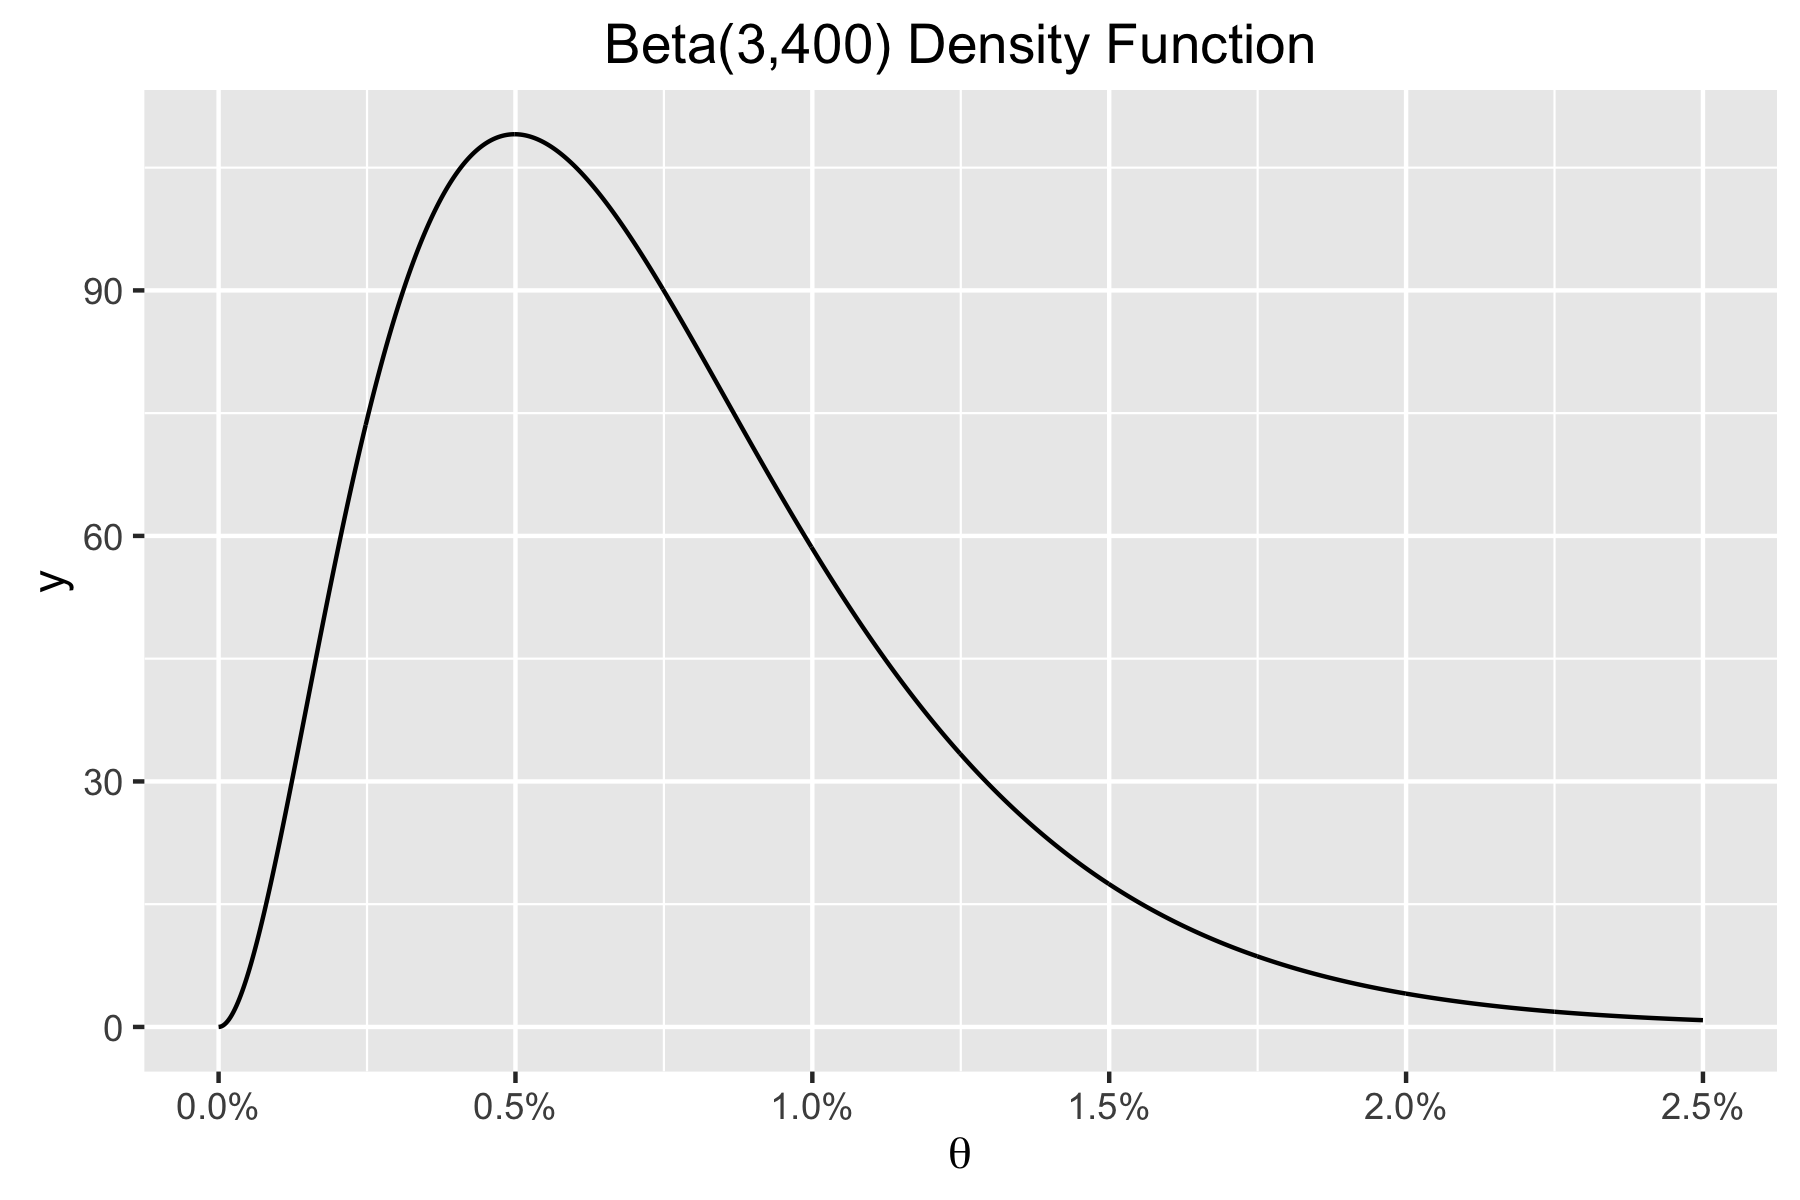
\includegraphics[height=2in]{figures/beta3-400}
\par\end{center}

In this basic Bayesian approach, the parameters $3$ and $400$ would
be chosen by the data scientist based on prior experience, or ``best
guess'', but without looking at the new data. Another approach would
be to use the data to help you choose the parameters $a$ and $b$
in $\mbox{Beta}(a,b)$. This would \textbf{not} be a Bayesian approach,
though it is frequently used in practice. One method in this direction
is called \textbf{empirical Bayes}. Empirical Bayes can be considered
a frequentist approach, in which we estimate $a$ and $b$ from the
data $\cd$ using some estimation technique, such as maximum likelihood.
The proper Bayesian approach to this type of thing is called \textbf{hierarchical
Bayes}, in which we put another prior distribution on $a$ and $b$.
We'll investigate each of these approaches below. 

\subsubsection*{Mathematical Description}

We'll now give a mathematical description of our model, assuming the
prior parameters $a$ and $b$ are directly chosen by the data scientist.
Let $n_{1},\ldots,n_{d}$ be the number of impressions we observe
for each of the $d$ apps. In this problem, we will not consider these
to be random numbers. For the $i$th app, let $c_{i}^{1},\ldots,c_{i}^{n_{i}}\in\left\{ 0,1\right\} $
be indicator variables determining whether or not each impression
was clicked. That is, $c_{i}^{j}=\ind{j\mbox{th impression on }i\mbox{th app was clicked}}$.
We can summarize the data on the $i$th app by $\cd_{i}=\left(x_{i},n_{i}\right)$,
where $x_{i}=\sum_{j=1}^{n_{i}}c_{i}^{j}$ is the total number of
impressions that were clicked for app $i$. Let $\theta=(\theta_{1},\ldots,\theta_{d})$,
where $\theta_{i}$ is the CTR for app $i$. 

In our Bayesian approach, we act as though the data were generated
as follows:
\begin{enumerate}
\item Sample $\theta_{1},\ldots,\theta_{d}$ i.i.d. from Beta$(a,b)$. 
\item For each app $i$, sample $c_{i}^{1},\ldots,c_{i}^{n_{i}}$ i.i.d.
from Bernoulli$(\theta_{i})$. 
\end{enumerate}

\subsection{{[}Optional{]} \label{subsec:Empirical-Bayes-single-app}Empirical
Bayes for a single app}

We start by working out some details for Bayesian inference for a
single app. That is, suppose we only have the data $\cd_{i}$ from
app $i$, and nothing else. Mathematically, this is exactly the same
setting as the coin tossing setting above, but here we push it further.
\begin{enumerate}
\item Give an expression for $p(\cd_{i}\mid\theta_{i})$, the likelihood
of $\cd_{i}$ given the probability of click $\theta_{i}$, in terms
of $\theta_{i}$, $x_{i}$ and $n_{i}$.\\
\item We will take our prior distribution on $\theta_{i}$ to be $\mbox{Beta}(a,b)$.
The corresponding probability density function is given by
\[
p(\theta_{i})=\mbox{Beta}(\theta_{i};a,b)=\frac{1}{B(a,b)}\theta_{i}^{a-1}\left(1-\theta_{i}\right)^{b-1},
\]
where $B(a,b)$ is called the Beta function. Explain (without calculation)
why we must have
\[
\int\theta_{i}^{a-1}\left(1-\theta_{i}\right)^{b-1}\,d\theta_{i}=B(a,b).
\]
\\
\item Give an expression for the posterior distribution $p(\theta_{i}\mid\cd_{i})$.
In this case, include the constant of proportionality. In other words,
do not use the ``is proportional to'' sign $\propto$ in your final
expression. You \textbf{may }reference the Beta function defined above.
{[}Hint: This problem is essentially a repetition of an earlier problem.{]} 
\item Give a closed form expression for $p(\cd_{i})$, the marginal likelihood
of $\cd_{i}$, in terms of the $a,b,x_{i},$ and $n_{i}$. You may
use the normalization function $B(\cdot,\cdot)$ for convenience,
but you should not have any integrals in your solution. (Hint: $p(\cd_{i})=\int p\left(\cd_{i}\mid\theta_{i}\right)p(\theta_{i})\,d\theta_{i}$,
and the answer will be a ratio of two beta function evaluations.)
\item The maximum likelihood estimate for $\theta_{i}$ is $x_{i}/n_{i}$.
Let $p_{\text{MLE}}(\cd_{i})$ be the marginal likelihood of $\cd_{i}$
when we use a prior on $\theta_{i}$ that puts all of its probability
mass at $x_{i}/n_{i}$. Note that 
\begin{eqnarray*}
p_{\text{MLE}}(\cd_{i}) & = & p\left(\cd_{i}\mid\theta_{i}=\frac{x_{i}}{n_{i}}\right)p\left(\theta_{i}=\frac{x_{i}}{n_{i}}\right)\\
 & = & p\left(\cd_{i}\mid\theta_{i}=\frac{x_{i}}{n_{i}}\right).
\end{eqnarray*}
Explain why, or prove, that $p_{\text{MLE}}(\cd_{i})$ is larger than
$p(\cd_{i})$ for any other prior we might put on $\theta_{i}$. If
it's too hard to reason about all possible priors, it's fine to just
consider all Beta priors. {[}Hint: This does not require much or any
calculation. It may help to think about the integral $p(\cd_{i})=\int p\left(\cd_{i}\mid\theta_{i}\right)p(\theta_{i})\,d\theta_{i}$
as a weighted average of $p(\cd_{i}\mid\theta_{i})$ for different
values of $\theta_{i}$, where the weights are $p(\theta_{i})$.{]}
\item One approach to getting an \textbf{empirical Bayes} estimate of the
parameters $a$ and $b$ is to use maximum likelihood. Such an empirical
Bayes estimate is often called an \textbf{ML-2} estimate, since it's
maximum likelihood, but at a higher level in the Bayesian hierarchy.
To emphasize the dependence of the likelihood of $\cd_{i}$ on the
parameters $a$ and $b$, we'll now write it as $p(\cd_{i}\mid a,b)$\footnote{Note that this is a slight (though common) abuse of notation, because
$a$ and $b$ are not random variables in this setting. It might be
more appropriate to write this as $p(\cd_{i};a,b)$ or $p_{a,b}(\cd_{i})$.
But this isn't very common.}. The empirical Bayes estimates for $a$ and $b$ are given by
\[
(\hat{a},\hat{b})=\argmax_{\left(a,b\right)\in(0,\infty)\times(0,\infty)}p(\cd_{i}\mid a,b).
\]
To make things concrete, suppose we observed $x_{i}=3$ clicks out
of $n_{i}=500$ impressions. A plot of $p(\cd_{i}\mid a,b)$ as a
function of $a$ and $b$ is given in Figure \ref{fig:single-app-contour-plot}.
\begin{figure}
\centering{}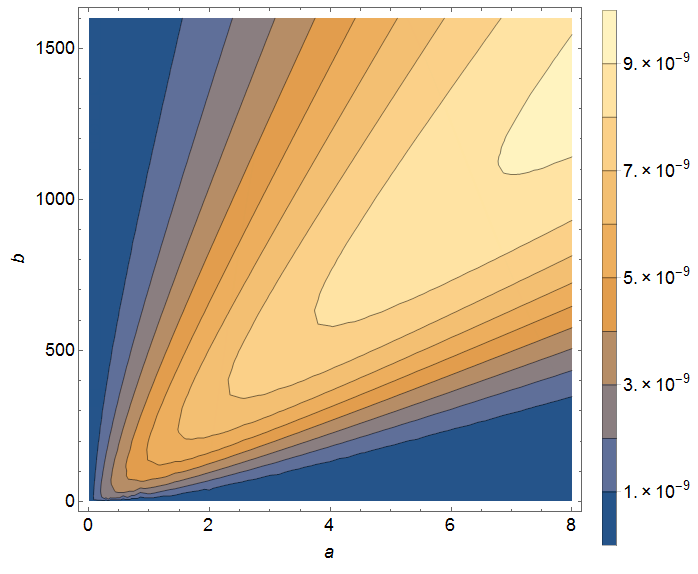
\includegraphics[height=2.5in]{figures/single-app-marginal-lik-contour-plot}\caption{\label{fig:single-app-contour-plot}A plot of $p(\protect\cd_{i}\mid a,b)$
as a function of $a$ and $b$. }
\end{figure}
It appears from this plot that the likelihood will keep increasing
as $a$ and $b$ increase, at least if $a$ and $b$ maintain a particular
ratio. Indeed, this likelihood function never attains its maximum,
so we cannot use ML-2 here. Explain what's happening to the prior
as we continue to increase the likelihood. {[}Hint: It is a property
of the Beta distribution (not difficult to see), that for any $\theta\in\left(0,1\right)$,
there is a Beta distribution with expected value $\theta$ and variance
less than $\eps$, for any $\eps>0$. What's going in here is similar
to what happens when you attempt to fit a gaussian distribution $\cn(\mu,\sigma^{2})$
to a single data point using maximum likelihood.{]}
\end{enumerate}

\subsection{{[}Optional{]} \label{subsec:Empirical-Bayes-multiple-apps}Empirical
Bayes Using All App Data}

In the previous section, we considered working with data from a single
app. With a fixed prior, such as Beta(3,400), our Bayesian estimates
for $\theta_{i}$ seem more reasonable to me\footnote{I say ``to me'', since I am the one who chose the prior. You may
have an entirely different prior, and think that my estimates are
terrible.} than the MLE when our sample size $n_{i}$ is small. The fact that
these estimates seem reasonable is an immediate consequence of the
fact that I chose the prior to give high probability to estimates
that seem reasonable to me, before ever seeing the data. Our earlier
attempt to use empirical Bayes (ML-2) to choose the prior in a data-driven
way was not successful. With only a single app, we were essentially
overfitting the prior to the data we have. In this section, we'll
consider using the data from all the apps, in which case empirical
Bayes makes more sense.
\begin{enumerate}
\item Let $\cd=\left(\cd_{1},\ldots,\cd_{d}\right)$ be the data from all
the apps. Give an expression for $p(\cd\mid a,b)$, the \textbf{marginal
likelihood} of $\cd$. Expression should be in terms of $a,b,x_{i},n_{i}$
for $i=1,\ldots,d$. Assume data from different apps are independent.
(Hint: This problem should be easy, based on a problem from the previous
section.) 
\item Explain why $p(\theta_{i}\mid\cd)=p(\theta_{i}\mid\cd_{i})$, according
to our model. In other words, once we choose values for parameters
$a$ and $b$, information about one app does not give any information
about other apps.
\item Suppose we have data from 6 apps. 3 of the apps have a fair number
of impressions, and 3 have relatively few. Suppose we observe the
following:\\
\begin{tabular}{|c|c|c|}
\hline 
 & Num Clicks & Num Impressions\tabularnewline
\hline 
\hline 
App 1 & 50 & 10000\tabularnewline
\hline 
App 2 & 160 & 20000\tabularnewline
\hline 
App 3 & 180 & 60000\tabularnewline
\hline 
App 4 & 0 & 100\tabularnewline
\hline 
App 5 & 0 & 5\tabularnewline
\hline 
App 6 & 1 & 2\tabularnewline
\hline 
\end{tabular}\\
Compute the empirical Bayes estimates for $a$ and $b$. (Recall,
this amounts to computing $(\hat{a},\hat{b})=\argmax_{\left(a,b\right)\in\reals^{>0}\times\reals^{>0}}p(\cd\mid a,b).$)
This will require solving an optimization problem, for which you are
free to use any optimization software you like (perhaps \href{https://docs.scipy.org/doc/scipy/reference/optimize.html}{scipy.optimize}
would be useful). The empirical Bayes prior is then Beta$(\hat{a},\hat{b})$,
where $\hat{a}$ and $\hat{b}$ are our ML-2 estimates. Give the corresponding
prior mean and standard deviation for this prior.
\item Complete the following table:\\
\begin{tabular}{|c|c|c|c|c|c|c|}
\hline 
 & NumClicks & NumImpressions & MLE & MAP & PosteriorMean & PosteriorSD\tabularnewline
\hline 
\hline 
App 1 & 50 & 10000 & 0.5\%  &  &  & \tabularnewline
\hline 
App 2 & 160 & 20000 & 0.8\%  &  &  & \tabularnewline
\hline 
App 3 & 180 & 60000 & 0.3\%  &  &  & \tabularnewline
\hline 
App 4 & 0 & 100 & 0\%  &  &  & \tabularnewline
\hline 
App 5 & 0 & 5 & 0\%  &  &  & \tabularnewline
\hline 
App 6 & 1 & 2 & 50\%  &  &  & \tabularnewline
\hline 
\end{tabular}\\
Make sure to take a look at the PosteriorSD values and note which
are big and which are small.
\end{enumerate}

\subsection{{[}Optional{]} Hierarchical Bayes}

In Section \ref{subsec:Empirical-Bayes-multiple-apps} we managed
to get empirical Bayes ML-II estimates for $a$ and $b$ by assuming
we had data from multiple apps. However, we didn't really address
the issue that ML-II, as a maximum likelihood method, is prone to
overfitting if we don't have enough data (in this case, enough apps).
Moreover, a true Bayesian would reject this approach, since we're
using our data to determine our prior. If we don't have enough confidence
to choose parameters for $a$ and $b$ without looking at the data,
then the only proper Bayesian approach is to put another prior on
the parameters $a$ and $b$. If you are very uncertain about values
for $a$ and $b$, you could put priors on them that have high variance. 
\begin{enumerate}
\item {[}Optional{]} Suppose $P$ is the Beta$(a,b)$ distribution. Conceptually,
rather than putting priors on $a$ and $b$, it's easier to reason
about priors on the mean $m$ and the variance $v$ of $P$. If we
parameterize $P$ by its mean $m$ and the variance $v$, give an
expression for the density function $\mbox{Beta}(\theta;m,v)$. You
are free to use the internet to get this expression -- just be confident
it's correct. {[}Hint: To derive this, you may find it convenient
to write some expression in terms of $\eta=a+b$.{]}
\item {[}Optional{]} Suggest a prior distribution to put on $m$ and $v$.
{[}Hint: You might want to use one of the distribution families given
\href{https://davidrosenberg.github.io/mlcourse/Archive/2016/Lectures/10b.conditional-probability-models.pdf\#page=6}{in this lecture}.
\item {[}Optional{]} Once we have our prior on $m$ and $v$, we can go
``full Bayesian'' and compute posterior distributions on $\theta_{1},\ldots,\theta_{d}$.
However, these no longer have closed forms. We would have to use approximation
techniques, typically either a Monte Carlo sampling approach or a
variational method, which are beyond the scope of this course\footnote{If you're very ambitious, you could try out a package like \href{https://pystan.readthedocs.io/en/latest/}{PyStan}
to see what happens.}. After observing the data $\mbox{\ensuremath{\cd}}$, $m$ and $v$
will have some posterior distribution $p(m,v\mid\cd)$. We can approximate
that distribution by a point mass at the mode of that distribution
$\left(m_{\text{MAP}},v_{\text{MAP}}\right)=\argmax_{m,v}p(m,v\mid\cd)$.\textbf{
Give expressions} for the posterior distribution $p(\theta_{1},\ldots,\theta_{d}\mid\cd)$,
with and without this approximation. You do not need to give any explicit
expressions here. It's fine to have expressions like $p(\theta_{1},\ldots,\theta_{d}\mid m,v)$
in your solution. Without the approximation, you will probably need
some integrals. It's these integrals that we need sampling or variational
approaches to approximate. While one can see this approach as a way
to approximate the proper Bayesian approach, one could also be skeptical
and say this is just another way to determine your prior from the
data. The estimators $\left(m_{\text{MAP}},v_{\text{MAP}}\right)$
are often called \textbf{MAP-II estimators}, since they are MAP estimators
at a higher level of the Bayesian hierarchy. 
\end{enumerate}

\end{document}
